\section{Experiment Results}

As an analysis tool, the TL-HMM model provides with us the following two
patterns to characterize student behavior:
\begin{enumerate*}[label=(\arabic*)]
  \item the latent state representations, and
  \item the latent state transitions.
\end{enumerate*}
Thus to evaluate the proposed model, we conduct experiments to
qualitatively analyze both types of patterns discovered from empirical MOOC
log data. Specifically, we look at the MOOC logs associated with the
\textretrieval{} Coursera MOOC offered by \UIUC{}.
Table~\ref{table:datasets} provides statistics about the sequences we
extracted from this MOOC and the action space we used for those sequences.

\begin{marginfigure}
  %\vspace{-2in}
  \centering
  \begin{subfigure}[t]{\textwidth}
    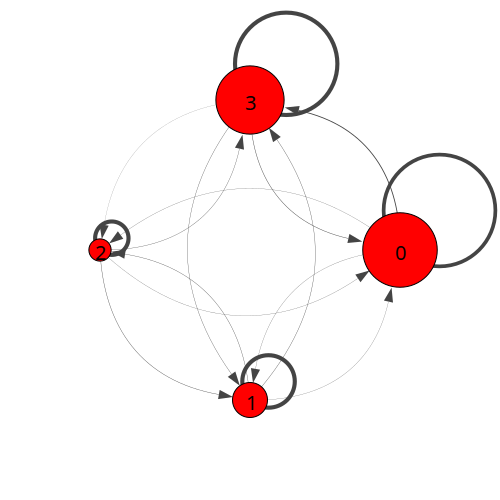
\includegraphics[width=0.95\textwidth,trim={0 3cm 0 2cm}]{../figures/trans-comp/trans-avg.png}
    \caption{\vspace{20pt}\label{fig:trans-avg}}
  \end{subfigure}

  \begin{subfigure}[t]{\textwidth}
    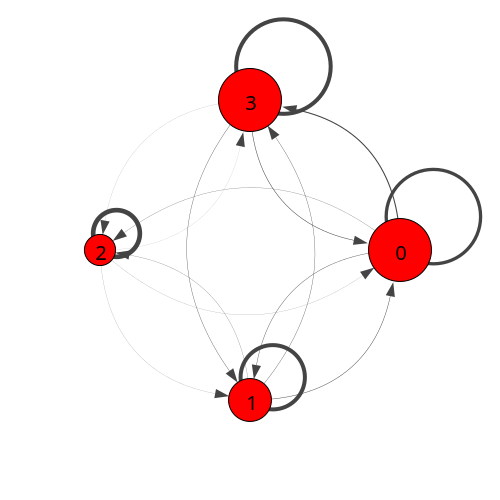
\includegraphics[width=0.95\textwidth,trim={0, 3cm 0 2cm}]{../figures/trans-comp/trans-perfect.png}
    \caption{\vspace{20pt}\label{fig:trans-perfect}}
  \end{subfigure}

  \begin{subfigure}[t]{\textwidth}
    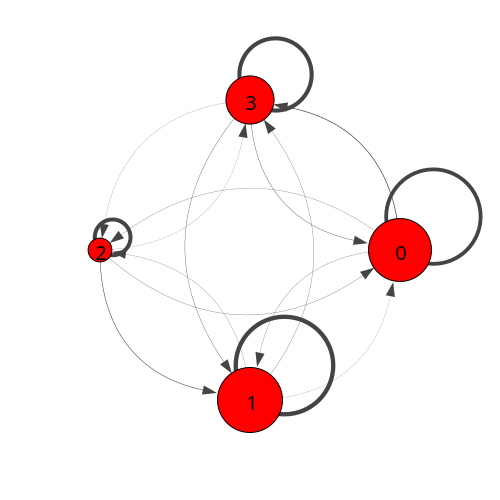
\includegraphics[width=0.95\textwidth,trim={0, 3cm 0 2cm}]{../figures/trans-comp/trans-low.png}
    \caption{\label{fig:trans-low}}
  \end{subfigure}

  \caption{The latent state transition diagrams for a 4-state TL-HMM fit to
  \protect\textretrieval{} for all students (a) compared to only ``perfect''
  students (b) and only ``low'' students (c).}
  \label{fig:trans-comp}
\end{marginfigure}

\begin{figure*}
  \centering
  \begin{subfigure}[t]{0.24\textwidth}
    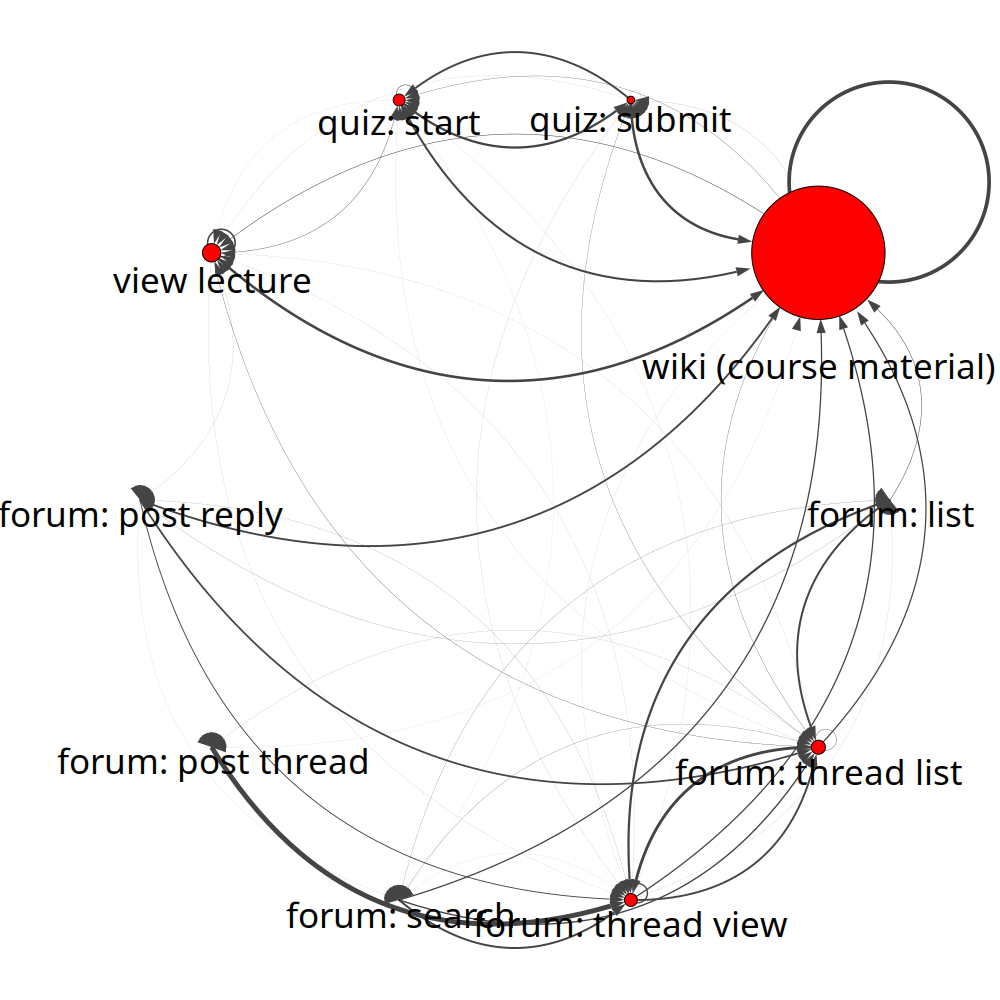
\includegraphics[width=\textwidth]{../figures/text-4state/state0.png}
    \caption{\label{fig:state0}State 0}
  \end{subfigure}
  \begin{subfigure}[t]{0.24\textwidth}
    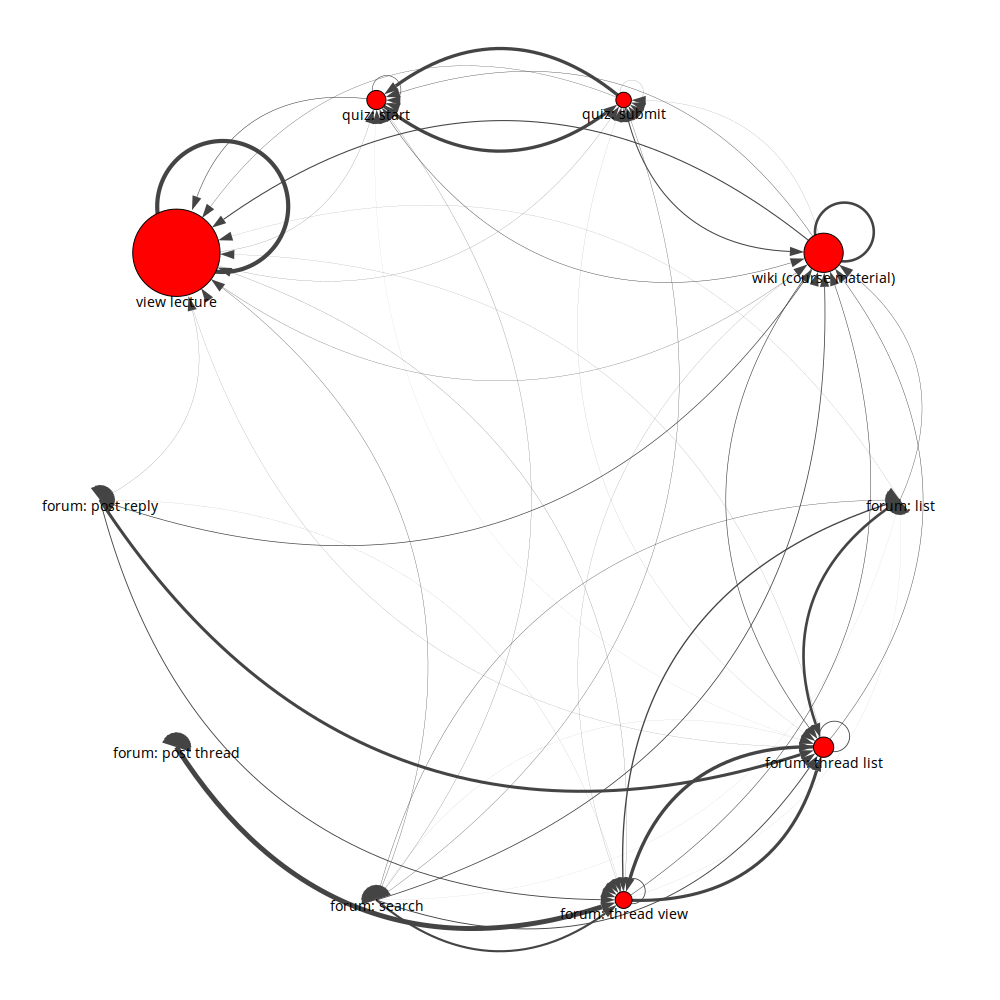
\includegraphics[width=\textwidth]{../figures/text-4state/state1.png}
    \caption{\label{fig:state1}State 1}
  \end{subfigure}
  \begin{subfigure}[t]{0.24\textwidth}
    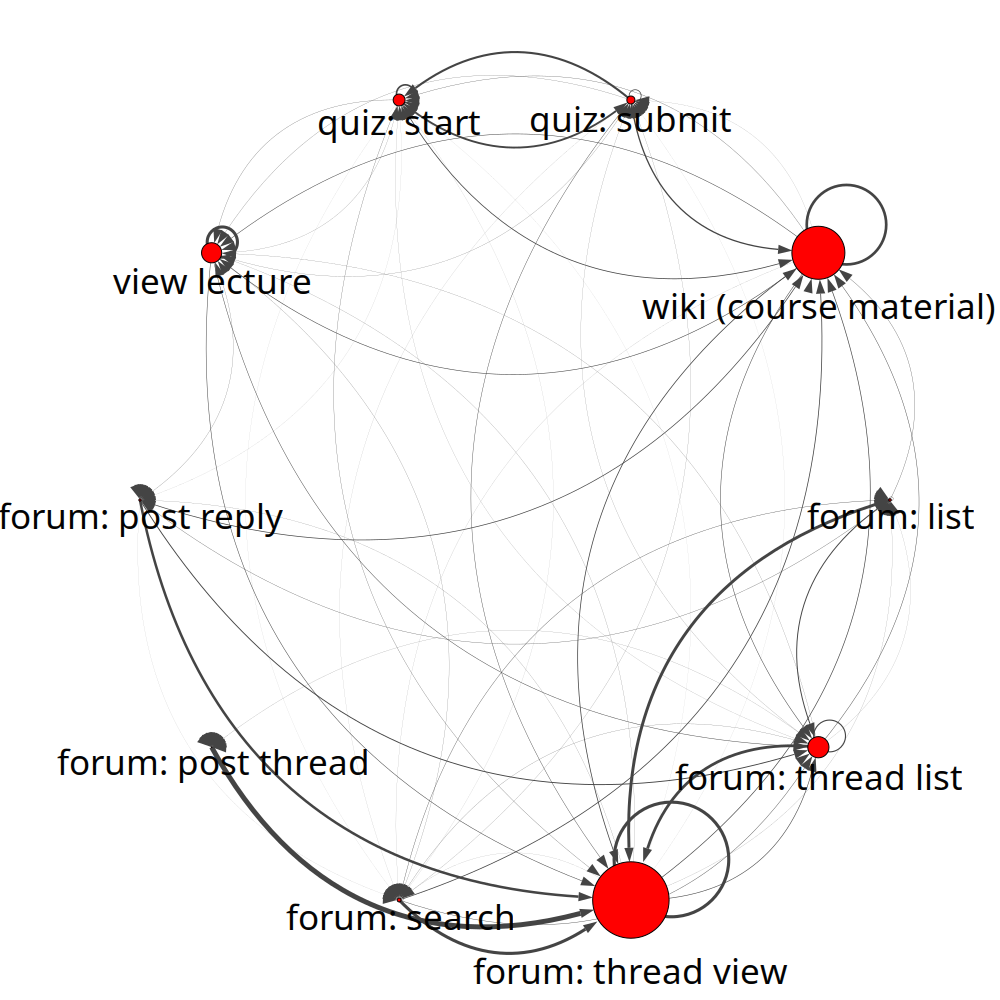
\includegraphics[width=\textwidth]{../figures/text-4state/state2.png}
    \caption{\label{fig:state2}State 2}
  \end{subfigure}
  \begin{subfigure}[t]{0.24\textwidth}
    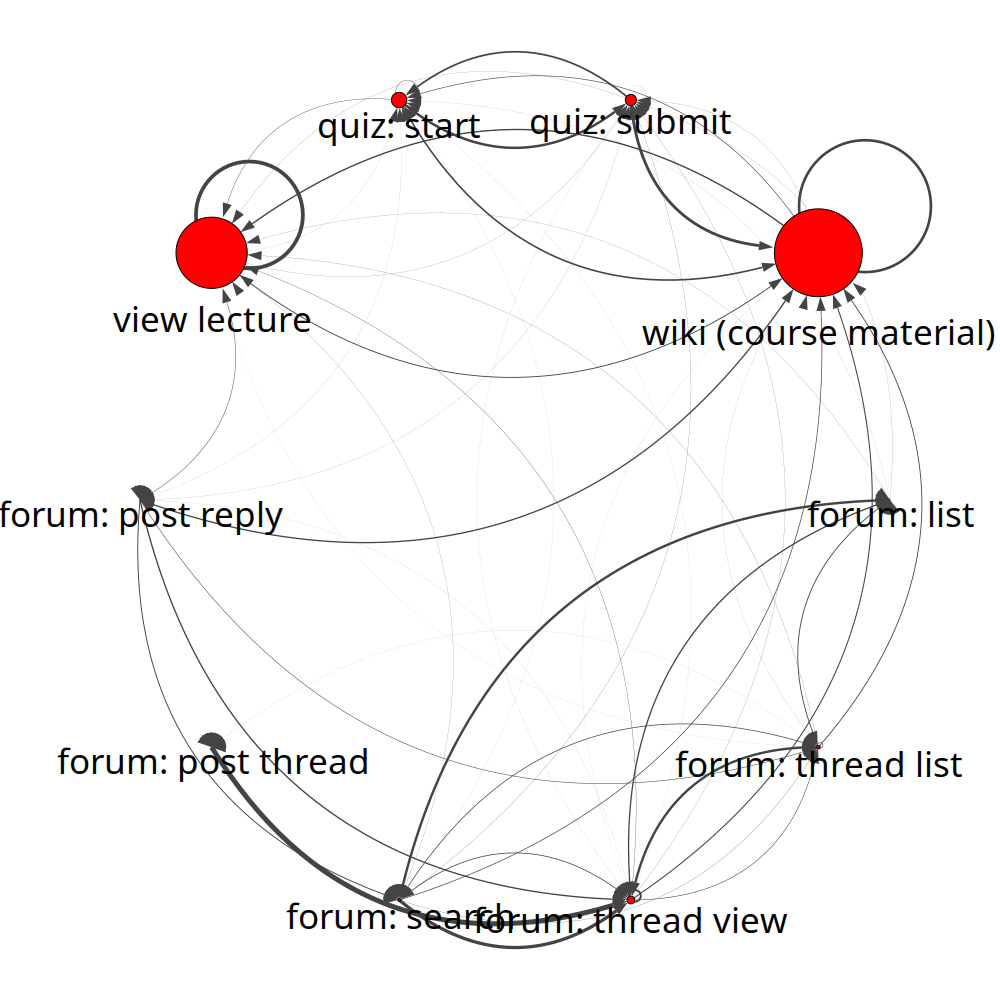
\includegraphics[width=\textwidth]{../figures/text-4state/state3.png}
    \caption{\label{fig:state3}State 3}
  \end{subfigure}
  \caption{Example states learned by a 4-state TL-HMM.}
  \label{fig:states}
\end{figure*}

To visualize the Markov models that represent our latent states, we plot
them as a directed graph where we set the size of a node to be proportional
to its probability of being visited during a random walk.  We let the
thickness of a directed edge $(u, v)$ reflect the probability of taking
that edge given that a random walk is currently at note $u$ (as indicated
by the transition matrix). Figure~\ref{fig:states} shows the four latent
states we learned by fitting a 4-state TL-HMM to the \textretrieval{}
sequence dataset.

A unique property of our model is its ability to capture transitions
between the \emph{behavior patterns themselves} that are captured by the
latent states. In Figure~\ref{fig:trans-avg} we show the latent state
transition diagram for the 4-state TL-HMM we learned.
We can see that the ``forum browsing'' state 2 (figure~\ref{fig:state2})
has relatively lower probability than the other states as we might expect.
It also makes sense that state 0 (figure~\ref{fig:state0}) has rather high
probability as this state likely captures all sequences where a student
logged in to the platform and then did nothing else (likely checking for
updates). If we look at state 1 (figure~\ref{fig:state1}) and state 3
(figure~\ref{fig:state3}), their relative probabilities match our intuition
as well. State 1 seems to capture a more engaged browsing session, where
there is non-negligible probability associated with different activities
such as quiz taking and forum browsing and, importantly, these activities
have high probability symmetric edges (so students are taking quizzes one
after the other, or viewing forum threads in succession). By contrast,
state 3 seems to capture a more passive student, with negligible
probability mass associated with forum activity (with low symmetry in the
edges). The link between ``quiz submit'' and ``quiz start'' (indicating
quiz repetition) is also significantly lower than state 1.

Thus, we might expect to see students that perform well in the course
preferring states 1 and 2 over states 0 and 3. To verify this, we took the
model we learned on the full training data and retrofit it to training data
consisting only of sequences produced by students that had perfect marks.
To prevent the latent state meanings from drifting, we forced the model
parameters associated with their Markov model representations to be fixed,
in effect only learning initial and transition probabilities for the top
layer of our TL-HMM.\ We show the updated latent state transition diagram
in Figure~\ref{fig:trans-perfect}. We can see that the probability of state
2 has increased dramatically, while the probability of states 0 and 3 has
decreased. State 1 had its probability increase, but only very slightly.

In Figure~\ref{fig:trans-low} we plot the latent state transition diagram
for a second group of ``low'' students. These students were selected so
that they attempted all required quizzes in the course, but such that their
average quiz score was $\leq 70\%$. Here, we see that \emph{state 1} has a
large increase in size, where we might have expected state 3 to grow
instead.  However, there is an alternative explanation for this phenomenon.
Since state 1 seems to indicate a highly engaged student, it is a perfectly
reasonable explanation for the ``low'' student group as they are going to
be working hard to try to fill in the gaps in their knowledge. By contrast,
the ``perfect'' student group likely has many members who can take the quiz
more passively and get perfect marks, perhaps because they already know
much of the material being presented, or are just naturally strong and do
not require much background review to perform well. This also explains why
state 1 did not increase in size for the ``perfect'' group like we were
anticipating. Our model lends itself well to discovering this potentially
counter-intuitive insight.
